\documentclass{cmc}

\begin{document}

\pagestyle{fancy}
\lhead{\textit{\textbf{Computational Motor Control, Spring 2019} \\
    Python exercise, Lab 5, GRADED}} \rhead{Student \\ Aurélien Morel, Lucas Wälti, Luca Kiener}

\section*{Student names: Aurélien Morel, Lucas Wälti, Luca Kiener}
\textit{Instructions: Update this file (or recreate a similar one,
  e.g.\ in Word) to prepare your answers to the questions. Feel free
  to add text, equations and figures as needed. Hand-written notes,
  e.g.\ for the development of equations, can also be included e.g.\
  as pictures (from your cell phone or from a scanner).
  \textbf{\corr{This lab is graded.}} and must be submitted before
  the \textbf{\corr{Deadline : 11-04-2018 Midnight}}.  \\ Please
  submit both the source file (*.doc/*.tex) and a pdf of your
  document, as well as all the used and updated Python functions in a
  single zipped file called \corr{lab5\_name1\_name2\_name3.zip} where
  name\# are the team member’s last names.  \corr{Please submit only
    one report per team!}}
\\

\textit{The file \fileref{lab\#.py} is provided to run all exercises
  in Python.
  % Each \fileref{exercise\#.py} can be run to run an exercise
  % individually.
  % The list of exercises and their dependencies are shown in
  % Figure~\ref{fig:files}.
  When a file is run, message logs will be printed to indicate
  information such as what is currently being run and and what is left
  to be implemented. All warning messages are only present to guide
  you in the implementation, and can be deleted whenever the
  corresponding code has been implemented correctly.}


% \textit{In this exercise, you will explore the different modeling
%   techniques that can be used to control a single joint and
%   segment. We initially start by exploring a single joint controlled
%   by a pair of antagonist spring like muscles and then extend the
%   model by adding dampers to it. These only represent the passive
%   dynamics observed in a real musculoskeletal system. To make the
%   behavior more realistic we then study more complex hill muscle model
%   in detail. }

%%%%%%%%%% TO BE ADDED [WIP] %%%%%%%%%%

\begin{figure}[ht]
  \centering 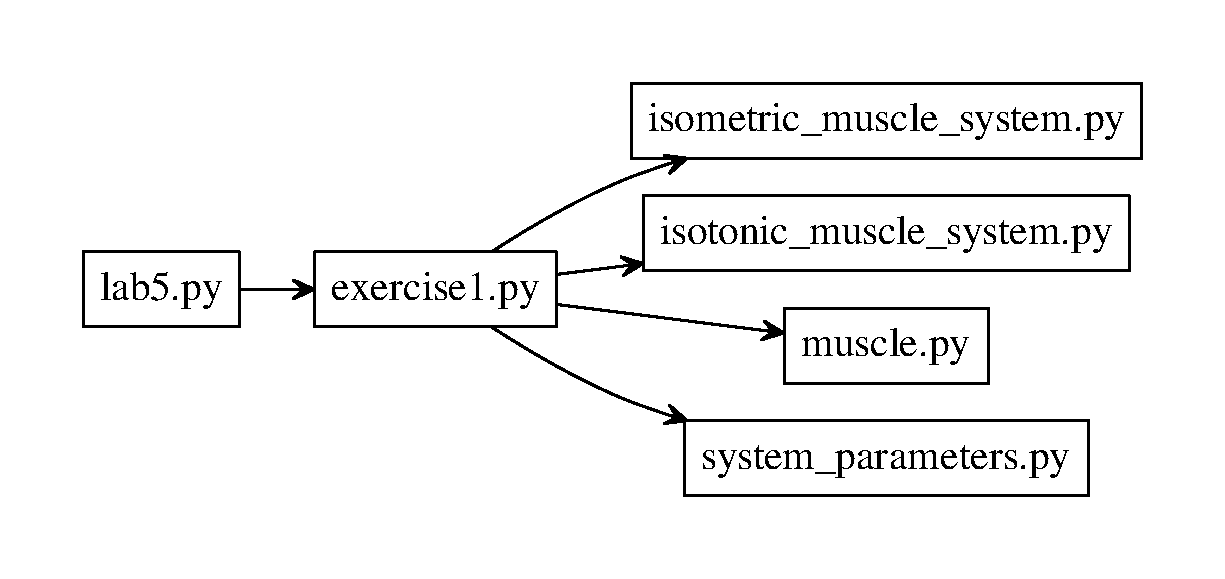
\includegraphics[width=0.5\textwidth]{figures/files}
  \caption{\label{fig:files} Exercise files dependencies. In this
  lab, you will be modifying \fileref{exercise1.py}.}
\end{figure}

\subsection*{Files to complete the exercises}
\label{sec:intro}

\begin{itemize}
\item \fileref{lab5.py} : Main file
\item \fileref{exercise1.py} : Main file to complete exercise 1
\item \fileref{system\_parameters.py} : Parameter class for Pendulum,
  Muscles and Neural Network (Create an instance and change properties
  using the instance. You do not have to modify the file)
\item \fileref{isometric\_muscle\_system.py} : Class to setup your
  isometric muscle test experiments
\item \fileref{isotonic\_muscle\_system.py} : Class to setup your
  isotonic muscle test experiments
\item \fileref{muscle.py} : Muscle class (You do not have to modify
  the file)
\end{itemize}

\textbf{NOTE : } '\textit{You do not have to modify}' does not mean
you should not, it means it is not necessary to complete the
exercises. But, \corr{you are expected to look into each of these
  files and understand how everything works}. You are free to explore
and change any file if you feel so.


\section*{Exercise 1 : Hill muscle model}
\label{sec:question-2}

Previous week you explored the role of different passive components
and the effects of its parameters on the system. In this exercise, we
try to understand the contractile or the active element of the hill
muscle model. The components of the hill muscle are described in
figure \ref{fig:hill_muscle}. The equations used to model the hill
muscle can be found in the pdf \fileref{HillMuscleEquations.pdf}

\begin{figure}[H]
  \centering 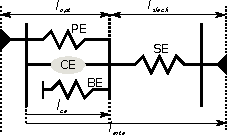
\includegraphics[scale=2.5]{figures/hill_muscle}
  \caption{Hill muscle model}
  \label{fig:hill_muscle}
\end{figure}

Where,

\begin{itemize}
\item $PE$ : Parallel element (Prevents muscle from over stretching)
\item $BE$ : Muscle Belly (Prevents muscle from collapsing on itself)
\item $SE$ : Series element or the muscle tendon element
\item $CE$ : Contractile Element or the active element
\item $l_{opt}$ : Muscle optimal fiber length
\item $l_{slack}$ : Muscle tendon slack length
\item $l_{CE}$ : Contractile element length
\item $l_{MTC}$ : Muscle Tendon Complex length
\end{itemize}


\begin{figure}[H]
  \centering
  \begin{subfigure}[b]{0.49\textwidth}
    { \centering
      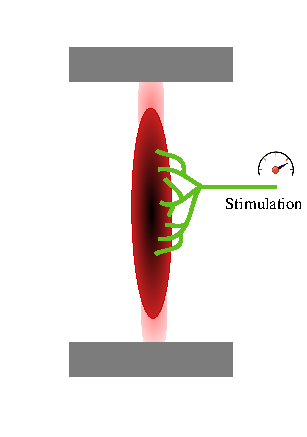
\includegraphics[width=\textwidth]{figures/isometric_muscle} }
    \caption{Isometric muscle setup :\\ To study the relationship
      between Force-Length.}
    \label{fig:isometric_muscle}
  \end{subfigure}
  \begin{subfigure}[b]{0.49\textwidth}
    { \centering
      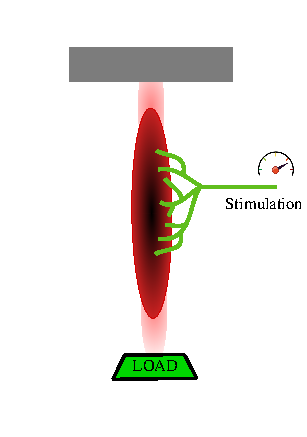
\includegraphics[width=\textwidth]{figures/isotonic_muscle} }
    \caption{Isotonic muscle setup :\\ To study the relationship
      between Force-Velocity.}
    \label{fig:isotonic_muscle}
  \end{subfigure}
  \caption{Muscle Length-Velocity-Force Setup}
  \label{fig:muscle-setup}
\end{figure}

\subsection*{Muscle Force-Length Relationship}
\label{sec:muscle-force-length}
In this exercise you will explore the relation between the length and
velocity of the muscle. In order to do this we replicate the set-up
show in figure \ref{fig:muscle-setup}.Here the length of the muscle is
held constant by attaching it's tendon to two fixed points. While
applying a constant stimulation, observing the force produced will
give the relationship between muscle contractile element length and
force.
\subsection*{1.a For a given stimulation, explore the relationship
  between active and passive muscle forces and the length of the
  contractile element.  Plot the force-length relationship curve.
  Discuss the different regions in the plot. Use the
  \fileref{isometric\_muscle\_system.py::IsometricMuscleSystem} instance
  to setup your experiment in \fileref{exercise1.py}}
  
Figure \ref{fig:1a} shows the different behaviour of the isometric muscle forces with increasing length and constant stimulation. First, when the total length is really small, the total force (i.e. tendon force) is close to zero. When increasing the length, the contractile element starts to apply some active force which contributes entirely to the total force. The maximal force of the contractile element is produced when its length $l_{CE}$ is equal to the muscles optimal fiber length $l_{opt}$: at this point the total force  reaches a local maximum. After the contractile element reached its peak force, it starts decreasing while the passive force starts increasing due to over-extension of the muscle-tendon complex. The lengthening of the muscle leads to high forces due to the passive elements while the active force becomes zero. 

\begin{figure}[H]
  \centering 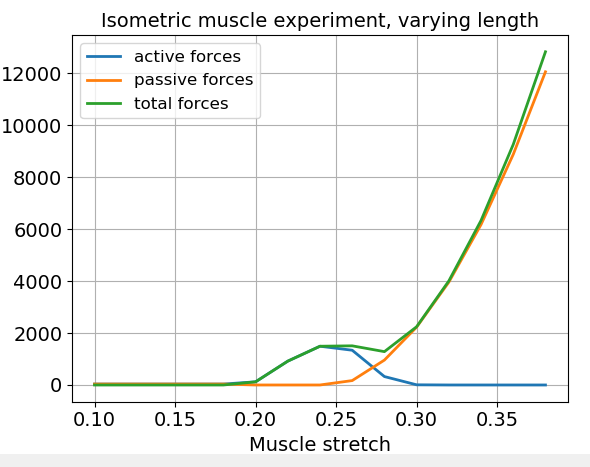
\includegraphics[scale=1]{figures/fig1}
  \caption{Isometric experimentation: varying length}
  \label{fig:1a}
\end{figure}

\subsection*{1.b In (1.a), you explored the muscle force-length
  relationship for a given stimulation. What happens to the
  relationship when the stimulation is varied between [0 - 1]? Support
  your response with one plot showing the different force-length
  relationship curves.}

The stimulation only influences the contractile element and hence the passive force remains the same, which dominate the total force at longer lengths. The higher the stimulation the larger the active force generated by the contractile element. In figure \ref{fig:2a}, you can see that, with increasing stimulation, the peak of the active force gets bigger. Logically, the decrease after the local peak gets smaller with smaller activation since the raising passive force can better compensate the decreasing active force, and there is no local peak for low stimulations. 
\begin{figure}[H]
  \centering 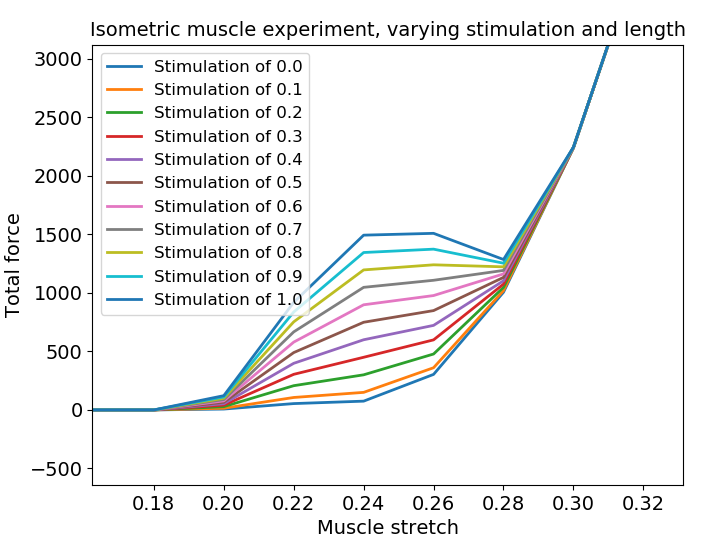
\includegraphics[scale=0.8]{figures/fig2}
  \caption{Isometric experimentation: varying stimulation}
  \label{fig:2a}
\end{figure}

\subsection*{1.c Describe how the fiber length ($l_{opt}$) influences
  the force-length curve.  (Compare a muscle comprised of short muscle
  fibers to a muscle comprised on long muscle fibers.). To change the
  parameter you can use
  \fileref{system\_parameters.py::MuscleParameters} before
  instantiating the muscle. No more than two plots are required. }
  
In figure \ref{fig:1c}, the force-length curves of the different fiber lengths ($l_{opt}$) are plotted. As expected, the fiber length influences the peak of active force. The peak is where the length of the contractile element is equal to the fiber length, as previously already mentioned. For shorter fiber lengths the active force maximum is reached earlier and vice versa. Also a change in fiber length causes a horizontal shift in the passive force-length relation.

\begin{figure}[ht]
  \begin{subfigure}[b]{0.48\textwidth}
    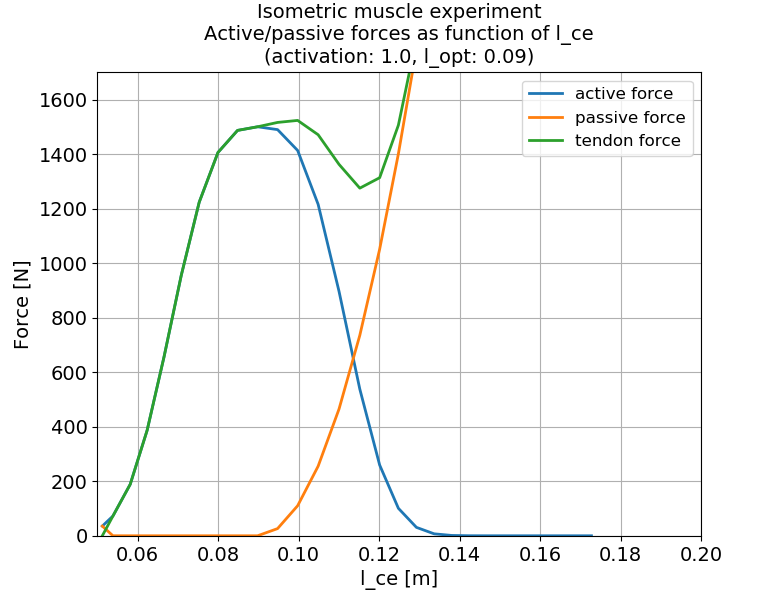
\includegraphics[width=\textwidth]{figures/passive_forces_as_function_of_l_ce_l_opt_09.png}
    \caption{Active/passive forces curve for $l_{opt} = 0.09$}
    \label{fig:}
  \end{subfigure}
  %
  \begin{subfigure}[b]{0.48\textwidth}
    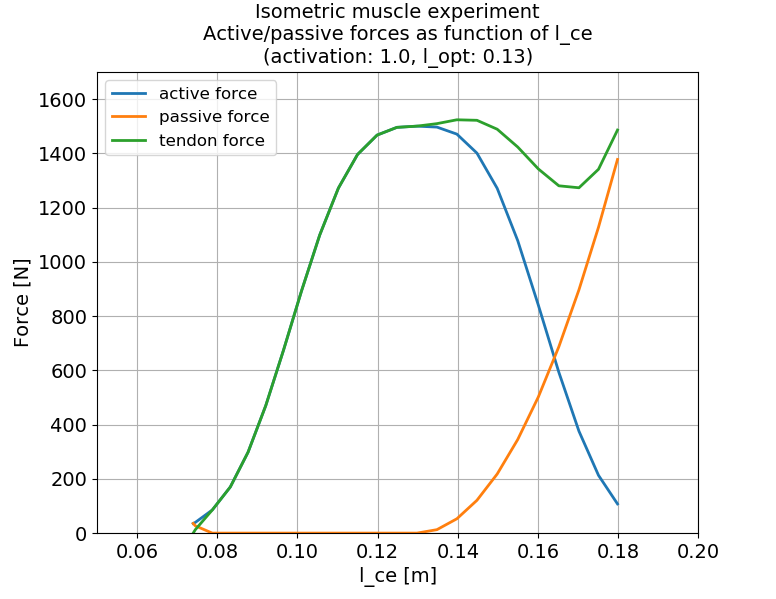
\includegraphics[width=\textwidth]{figures/passive_forces_as_function_of_l_ce_l_opt_13.png}
    \caption{Active/passive forces curve for $l_{opt} = 0.13$}
    \label{fig:}
  \end{subfigure}
  \caption{Fiber length's influence on force-length curve. The whole graph is shifted as well as scaled along the x axis depending on the value of $l_{opt}$.}
  \label{fig:1c}
\end{figure}


\subsection*{Muscle Velocity-Tension Relationship}
In this exercise you will explore the relation between the force and
velocity of the muscle. In order to do this we replicate the set-up
show in figure \ref{fig:muscle-setup}. Here the length of the muscle
is allowed to vary by attaching one of its end to a fixed point and
the other to a variable external load. While applying a constant load
initially and holding the muscle at constant length, a quick release
is performed to let the muscle contract and pull the weight. The
maximum velocity during this quick release will give us the
relationship between muscle contractile velocity and the force.


\corr{Note} : Since the velocity changes sign and you need to compute the maximum
velocity accordingly by checking if the muscle was stretched or compressed
at the end of the experiment.

\begin{equation}
  \label{eq:2}
 V_{ce} = \left\{
\begin{array}{ll}
      max(v_{ce}(t)) & l_{mtc} < (l_{opt} + l_{slack}) \\
      min(v_{ce}(t)) & else \\
\end{array}
\right.
\end{equation}

\subsection*{1.d For a stimulation of 1.0 and starting at optimal
  muscle length, explore the relationship between contractile element
  velocity and external load. Plot the Velocity-Tension relationship
  curve. Include shortening and lengthening regions. Use the
  \fileref{isotonic\_muscle\_system.py::IsotonicMuscleSystem} instance
  to setup your experiment in \fileref{exercise1.py}}
  
Figure \ref{fig:maxVel} shows that at low loads the muscle contracts since there is a positiv maximum velocity, which gets higher the lower the load. When the load gets to heavy for the muscle to contract, it stretches and maximum velocity becomes negativ, since the muscle tries to prevent further elongation. At large loads the maximum velocity asymptotically reaches a constant value of about -0.8m/s.

\begin{figure}[ht]
    \centering
    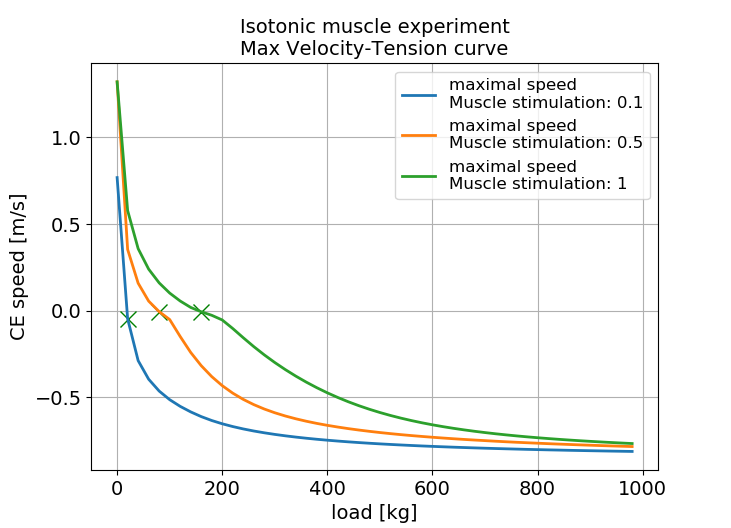
\includegraphics[width=0.6\textwidth]{figures/Max_Velocity-Tension_curve.png}
    \caption{Relationship between load and maximum achieved speed of the muscle. The curve on the left of the "$\times$" marker corresponds to the contraction motion, while the muscle elongates on the right of the marker. We also show the effect of different muscle stimulations.}
    \label{fig:maxVel}
\end{figure}

\subsection*{1.e For the muscle force-velocity relationship, why is
  the lengthening force greater than the force output during
  shortening? No plots necessary}

Because as already seen in the force-length plots, passive forces help the muscle at longer lengths and prevent it from over stretching.

\subsection*{1.f What happens to the force-velocity relationship
  when the stimulation is varied between [0 - 1]? Support your
  response with one plot showing the different force-velocity
  relationship curves.  }

As one can see in figure \ref{fig:maxVel}, the lower the stimulation the lower is the load under which the muscle still can contract. Additionally, since the force generated by the muscle is lower with lower stimulation the maximum velocity decreases more rapidly because this force can only bear smaller external loads.

\end{document}

